\begin{figure}[h]
	\centering
	\missingfigure{Klassendiagramm}		
	\caption{Klassendiagramm - A}
	\label{fig:klassendiagramm-a}
\end{figure}

\begin{table}[h]
	\centering
	\begin{tabularx}{\textwidth}{X X}
		\rowcolor[HTML]{C0C0C0} 
		\textbf{Klassenname} & \textbf{Aufgabe} \\
		Klasse A & Aufgabe A \\
		\rowcolor[HTML]{E7E7E7} 
		Klasse B & Aufgabe B \\
		Klasse C & Aufgabe C \\
		\rowcolor[HTML]{E7E7E7} 
		Klasse D & Aufgabe D \\
		Klasse E & Aufgabe E \\
		\rowcolor[HTML]{E7E7E7} 
		Klasse F & Aufgabe F \\
		Klasse G & Aufgabe G
	\end{tabularx}
	\caption{Klassenbeschreibung - A}
	\label{table:klassenbeschreibung-a}
\end{table}

\begin{tcolorbox}
Teilt eure Klassendiagramme bitte auf und baut \textbf{kein} einzelnes riesiges Diagramm.
Getter und Setter Methoden müssen hier nicht modelliert werden.
Sie sollten aber der klassischen Namenskonvention folgen, um die Nutzung in Sequenzdiagrammen zu ermöglichen.
\\\\
Auf jedes Diagramm folgt eine Tabelle, in der die Aufgabe \textbf{jeder} Klasse beschrieben wird.
\end{tcolorbox}

\section*{Klassendiagramm zur Android-App}

\begin{figure}[h]
	\centering
	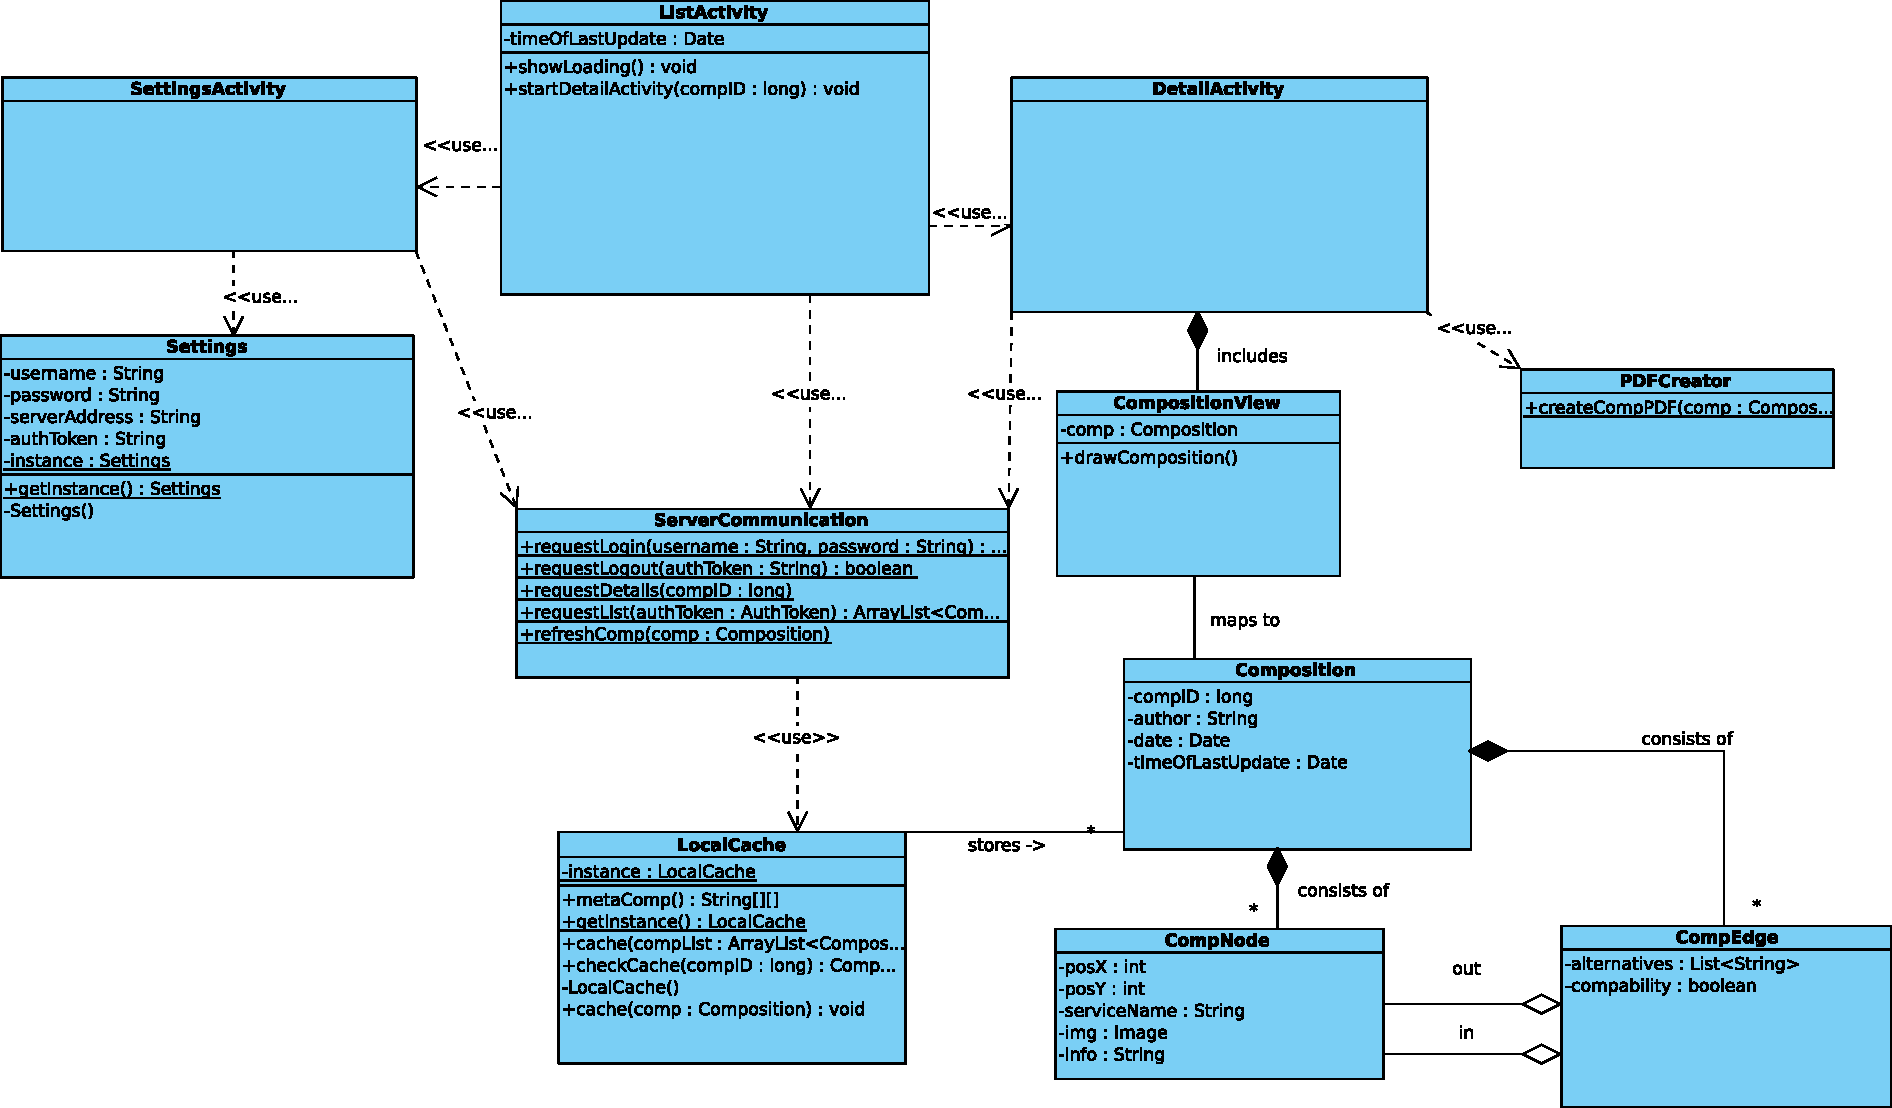
\includegraphics[width=\textwidth]{Klassendiagramm_App/Class_Diagram1}
	\caption{Klassendiagramm - App}
	\label{fig:klassendiagramm-a}
\end{figure}

\begin{table}[h]
	\centering
	\begin{tabularx}{\textwidth}{X X}
		\rowcolor[HTML]{C0C0C0} 
		\textbf{Klassenname} & \textbf{Aufgabe} \\
		ListActivity & MainActivity und Übersicht über sichtbare Kompositionen  \\
		\rowcolor[HTML]{E7E7E7} 
		SettingsActivity & Activity zum Festlegen von Einstellungen, zum Einloggen und Festlegen der Serveradresse \\
		DetailActivity & Detailansicht zur grafischen Darstellung einer Komposition \\
		\rowcolor[HTML]{E7E7E7} 
		Settings & Dient zur Kapselung der getroffenen Einstellungen \\
		CompositionView & Eigentliche View, in der das Zeichnen einer Komposition stattfindet. Jede DetailActivity verfügt über ein CompositionView. \\
		\rowcolor[HTML]{E7E7E7} 
		Composition & Interne Model-Abstraktion einer Komposition \\
		CompNode & Interne Model-Abstraktion eines Diensts, der als Knoten in einer Komposition fungiert. \\
		\rowcolor[HTML]{E7E7E7} 
		CompEdge & Interne Model-Abstraktion einer Kante zwischen zwei Diensten in einer Komposition \\
		PDFCreator & Helper-Klasse zur Generierung von PDFs, die Kompositionsbilder beinhalten. \\
			\rowcolor[HTML]{E7E7E7} 
		ServerCommunication & Anlaufpunkt für sämtliche Kommunikation mit dem Backend: ServerCommunication übernimmt daraufhin die Aufgabe, Verbindungen zum Server herzustellen, die Daten zu interpretieren und im richtigen Format weiterzugeben. \\
		LocalCache & Cache zur Speicherung von durch Anfragen erhaltenden Daten, damit diese nicht erneut angefragt werden müssen. 
	\end{tabularx}
	\caption{Klassenbeschreibung - App}
	\label{table:klassenbeschreibung-a}
\end{table}